\chapter{Design}\label{ch:Design}

This chapter looks at how the research artefact was designed to complete the research for this project and meet the aims and objectives laid out before.

\section{Methodology of the Research Artefact}
The chosen method for the development of the system is the iterative approach (Figure \ref{fig:ITA}). This allows for continuous development of the system. As seen below after the planning and research has taken place the implementation of the system can begin. Once this has finished, testing takes place, if the system does not meet requirements during the testing stage a second iteration of the development can start, and more implementation can take place
\begin{figure}[h!]
  \centering
  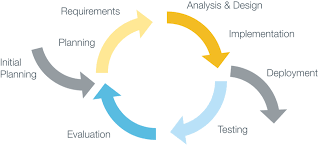
\includegraphics[width = (\textwidth)/2]{iterative.png}
  \caption{Diagram of the Iterative Approach}
  \label{fig:ITA}
\end{figure}\\

\section{Requirements of the Research Artefact}
\begin{itemize}
    \item The artefact needs to take an input of race data then produce an output of a predicted winner or non winner label based on the features of that horse.
    \item The artefact needs to correctly predict the winner to some acceptable degree of accuracy.
    \item The artefact could give and output of a probability of the horse winning as well as the predicted winner or non winner label 
    \item The artefact could allow for fresh race data so a prediction can be made on an upcoming race.
    
\end{itemize}

\section{Dataset Design}
During the literature review, data collection techniques were looked at as a way of building the data set. Whilst implementing a data scraper an observation of the data set built was that there wasn't enough data to train a model on, due to not being able to collect enough features to train the model off of. Because of this a decision was made to use a pre-existing data set. The data set is from \url{www.ukhorseracing.co.uk}. The data set before preprocessing has four hundred and seventy two features, and has 1,137,865 rows. The data contains over eighty thousand races from the past ten years for the model to be trained off of. Due to the size of the data set it was believed that a model could be trained to a higher accuracy then if the model had been trained off of a data set built from collected data via scraping.

\section{Model Design Approach}

The model will work in a similar way to the flowchart below ( Figure \ref{fig:FC}). As seen by the flowchart the research artefact software will view if the data needs preprocessing or not, then it will split the data, train the model, then predict the outcome. This is a very basic implementation as there is more sub processes that will take place and some may need to be implemented further on. An example of a sub process that was implemented further on was SMOTE, an oversampling technique to try and reduce over fitting in a machine learning model.
\begin{figure}[h!]
  \centering
  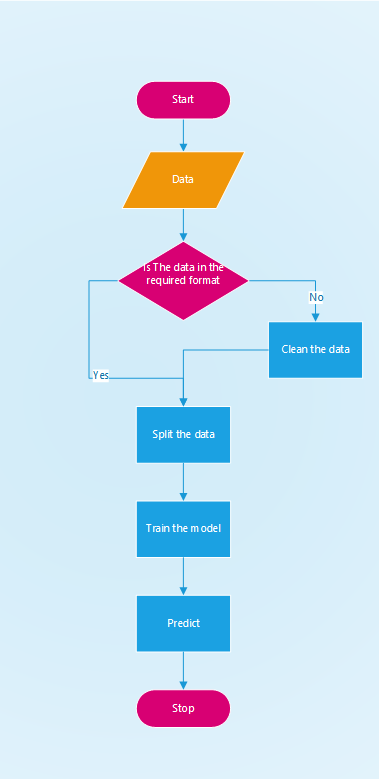
\includegraphics[width = (\textwidth)/2]{flowchart.png}
  \caption{Basic flowchart of model implementation}
  \label{fig:FC}
\end{figure}


\section{Conclusions}
In conclusion the aspects of design touched upon in this chapter have greatly aided the production of the research artefact software implementation. Without the designs discussed above the time taken to produce the research artefact software would have been considerably longer. 
